\setcounter{chapter}{9}
\chapter{Ускоряем perl. Расширяем «C».}
\section{Генерация XS модулей}
Чтобы сгенерировать XS модуль, необходимо знать каким образом был скомпилирован perl. Все XS модули должны быть скомпилированы также. Узнать это можно с помощью вызова:
\begin{minted}{bash}
% perl -V:make
make='dmake';
\end{minted}
В данном случае perl был скомпилирован для операционной системы windows с помощью dmake.

Утилита h2xs, которая идет в дистрибутиве perl, позволяет генерировать XS-интерфейс к коду на C. Параметр -b позволяет указывать минимальную версию perl, на которой предполагается запускать модуль, для целей обеспечения обратной совместимости. При этом, чем ниже указанная версия, тем больше <<обвязки>> будет строиться вокруг кода на C. Ключ -n позволяет указать используемый namespace, то есть полный путь к вашему пакету.

Если работающего кода пока нет, создать необходимый каркас для будущего модуля можно с помощью вызова:
\begin{minted}{bash}
% h2xs -b 5.10.1 -n local::sferamail::perlxs
\end{minted}
Будет создана директория со всеми нужными файлами для компиляции XS-модуля. Этот каркас можно было бы создать вручную, но так как требования к коду меняются от версии к версии, лучше всего это делать в автоматическом режиме. Если внутри данного каталога запустить утилиту make, скомпилируется пока пустой модуль.

Если программа на C уже написана, то сгенерировать XS-интерфейс можно указав путь к header-файлу с помощью той же утилиты:
\begin{minted}{bash}
h2xs -n local::sferamail::locale -O -x "F:\locale.h"
\end{minted}
В результате будет создана привязка к указанной библиотеке на C. Также можно будет сразу скопилировать XS модуль, после чего функции из библиотеки можно будет вызывать из perl. Базовый набор файлов, необходимых для создания модуля следующий:
\begin{description}[nosep, labelindent=2mm]
  \item[/ppport.h]--- файл, необходимый для обратной совместимости с другими версиями perl.
  \item[/lib/local/sferamail/perlxs.pm]--- файл, который нужно будет подключить в основной программе.
  \item[/perlxs.xs]--- файл, содержащий код XS модуля.
  \item[/fallback/const-c.inc и /fallback/const-xs.inc]: константы необходимые для работы в установленной версии perl. Эти файлы генерируются автоматически.
  \item[/Makefile.PL] Этот файл нужно исполнить на интерпретаторе perl, чтобы он создал обычный makefile и набор заголовочных файлов, которые совместимы с установленной версией perl.
  \item[/README]--- описание модуля
  \item[/t/local-sferamail-perlxs.t]--- тесты (опц.)
  \item[/Changes]--- история версий модуля
  \item[/MANIFEST]--- файл, содержащий список файлов в пакете.
\end{description} \noindent
Сборка и тестирование модуля выполняются с помощью команд:
\begin{minted}{bash}
% perl Makefile.PL
% dmake
% dmake test

t/sferamail-perlxs.t .. ok
All tests successful.
Files=1, Tests=1,  0 wallclock secs ( 0.00 usr +  0.08 sys =  0.08 CPU)
Result: PASS

% dmake install
\end{minted}
После этого скомпилированный модуль может быть использован.




\section{Макропроцессор}
На самом деле, код XS модуля отличается от привычного кода на C. На самом деле, XS является макро-языком для perl.
\begin{figure}[H] \centering
  \begin{tikzpicture}[
        entity/.style={ minimum height=1cm, minimum width=2.5cm, draw } ]
    \draw node[entity                      ] (XSU) {XSUBPP}
          node[entity,   right    = of XSU ] (C)   {C-File}
          node[entity,   below    = of C   ] (PM)  {PM-file}
          node[entity, below left = of XSU ] (XS)  {XS-file}
          node[entity, above left = of XSU ] (TM)  {TYPEMAP};
    \begin{scope}[line width = 1.2pt]
      \draw[-stealth] (PM) -- (C);
      \draw (C) -- (XSU) --+ (-2,0) edge (TM) edge (XS);
    \end{scope}
  \end{tikzpicture}
\end{figure} \noindent
А именно макрокомпилятору XSUBPP на вход подается XS-файл и TYPEMAP, то есть правила преобразования типов данных между C и perl, а в результате его выполнения макрокоманды расворачиваются в код на C. Именно этот получившийся файл компилируется компилятором языка C в файл с расширением so. Доступ к функциям из этого файла можно получить используя полученный ранее файл с расширением pm.

\section{Типы данных}
\subsection{Основные типы переменных}
Доступ к переменным perl из кода на C представляет из себя сложную задачу. Именно поэтому был создан макроязык XS, который позволяет приводить типы и работать со структурами данных perl. Однако понимать, как устроены структуры данных в perl необходимо, в том числе, и для целей отладки.

В perl существую следующие типы переменных:
\begin{itemize}[nosep]
  \item \textbf{SV}: Scalar Value
  \begin{itemize}[nosep]
    \item \textbf{IV}: signed integer value
    \item \textbf{UV}: unsigned integer value
    \item \textbf{NV}: double
    \item \textbf{PV}: pointer value
    \item \textbf{SV}
  \end{itemize}
  \item \textbf{AV}: Array Value
  \item \textbf{HV}: Hash Value
\end{itemize}
эти типы имеют одну и ту же структуру header'а, который представляет собой структуру из 4 значений:
\begin{figure}[H] \centering
\begin{tikzpicture}
\begin{simpleblock}[shift={(0,0)}]
	\add[color=blue!12, point]{ANY};
    \draw[line width=1pt, -latex] (R)+(1,0) node[anchor=west]{%
        Ссылка на данные из этой структуры данных}--(R);
	\add{REFCNT};
    \draw[line width=1pt, -latex] (R)+(1,0) node[anchor=west]{%
        Количество ссылок на эту структуру (нужно для работы сборщика мусора)
        }--(R);
	\add[width=0.75*3cm, flags] {FLAGS};
	\add[color=red!12, width=0.25*3cm, font = {\tiny}, toright] {\ TYPE};
	\add[point, color=blue!12] {SV\_U};
    \draw[line width=1pt, -latex] (R)+(1,0) node[anchor=west]{%
       SV\_U}--(R);
\end{simpleblock}
\end{tikzpicture}
\end{figure}\noindent
В FLAGS и TYPE хранится информация, характеризующая эту SV:
\begin{figure}[H] \centering
  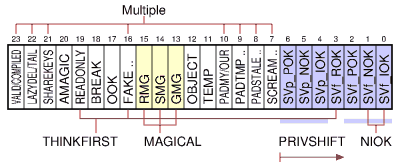
\includegraphics[width=10cm]{lectures/L10/flags.png}
\end{figure}\noindent
Помнить, какой бит флага что обозначает не требуется, так как они меняются от версии к версии perl. Поэтому необходимо использовать только именованные константы.

\subsection{Pointer Value}
Pointer Value (PV) --- одно из самых распространенных использований SV-ек в Perl, предназначенное для хранения строк. SvPV выглядит следующим образом:
\begin{figure}[H] \centering
	\begin{tikzpicture}[sv schemes]

		\begin{scope}[ shift={(-6,0)}, 	sv style=named SV,
			             scale=0.5,			setlabel=firstsv   	]
		    \draw (0,0.35) node {\bf svu\_pv};
		    \coordinate (temp2) at (1.5,3.5);
		\end{scope}

		\fill (firstsv-1) circle (0.7mm) (firstsv-2) circle (0.7mm);

		{ [shift=(temp2), xpv style = named xpv]
			\node {STASH};	 \node {MAGIC};	 \node {cur};	 \node {len};	}

		\draw[connect line] (firstsv-2) -- (xpv-1.west);


		{ [ shift= {($(xpv-1.east)+(4cm,0)$)},
			start chain=stack going right, anchor=west]
			\node [sn] {a}; \node [sn] {b};
			\node [sn] {c}; \node [sn] {};
			\node [sn] {x}; \node [sn] {y};
			\node [sn] {z}; \node [gsn] {\verb|\0|};
			\node [gsn] {}; \node [gsn] {C};     		}



		\draw[connect line] (firstsv-1)  --++ (0.25,0)
		  |- ++ (5.5,2.35) coordinate (temp2)  |- (stack-1.west);
		\draw[connect line, dashed] (temp2) --+ (0,-2.5) coordinate (temp3);

		{ [shift={(temp3)},start chain=hek going right,
			anchor=north east, xshift=-1cm]
			\node [sn wide] {hash};
			\node [sn wide] {len};
			\foreach \l in {s,h,a,r,e,d} \node [ysn] {\l};
			\node [gsn] {\verb|\0|};
			\node [sn wide] {flag};
		}

		\path [setcut=stack-4.center];

		\node [above=of stack-2] {\texttt{char[]}};
		\node [above=of hek-9  ] {\texttt{hek}};

	\end{tikzpicture}
\end{figure}
То есть в параметре \verb|SV_U| будет лежать ссылка на область памяти, где расположена строка, а по ссылке в параметре \verb|ANY| указана специальная структура, в которой хранится текущая длина строки (cur) и максимальная длина строки, для которой уже была выделена память (len). Perl всегда выделяет больше памяти, чем нужно для хранения строковой переменной, чтобы в большинстве случаев не было необходимости выделять дополнительную память при увеличении длины строки. Каждая строка в Perl должна заканчиваться нуль-байтом. Начиная с версии 5.18 в последний байт строки начали складывать количество ссылок на эту строку из перловых программ.


У SvPV есть флаг SvOOK, который обозначает, что у строки обрезано начало. В первом байте строки содержится число, которое указывает сколько байт строки нужно пропустить:
\begin{figure}[H] \centering % SvOOK
	\begin{tikzpicture}[sv schemes]

		\begin{scope}[shift={(-6,0)}, scale=0.5]
			\drawsv\draw (0,0.5) node {ARRAY};\drawsvflagbits
			\coordinate (temp1) at (2,0.5);
			\coordinate (temp2) at (1.5,3.5);
			\node[above] at (1.5,4) {\tt sv};
			\draw (-0.5,1.25) node {\tiny\bf POK, OOK};
		\end{scope}
		\fill (temp1) circle (0.7mm) (temp2) circle (0.7mm);

		{ [shift=(temp2), xpv style= named xpviv]
			\node {STASH};  \node {MAGIC};
			\node {cur}; 	  \node {len};
		}

		%\node[above, xshift=0.5cm, yshift=-0.1cm] at (xpviv-1.north) {\tt xpviv};

		\draw[connect line] (temp2) -- (xpviv-1.west);
		\path (xpviv-1.east)+(1.5cm,0) coordinate (temp3);


		{ [shift= {(temp3)},start chain=stack going right, anchor=west]
			\node [gsn] {2}; \node [gsn] {}; \node [sn] {c};\node [sn] {};
			\node [sn] {x};\node [sn] {y}; \node [sn] {z};
			\node [gsn] {\verb|\0|}; \node [gsn] {};\node [gsn] {};
			\node [above=of stack-9] {\texttt{char[]}};
			\path [setcut=stack-4.center];
		}
		\draw[connect line] (temp1) --++ (0.25,0) |- ++ (4,2.35) -| (stack-2.north east);

	\end{tikzpicture}
\end{figure}

\subsection{MAGIC} % TODO SvPVMG
С помощью флага MAGIC можно создавать переменные, у которых переопределены операции чтения, изменения и так далее. Если созданная SV-ка имеет такой флаг, в ней параметр ANY должен будет указывать на специальную структуру \verb|xpvmg| (см. схему ниже), у которой в свою очередь по ключу MAGIC указана другая структура ---  \verb|magic|. В структуре \verb|magic| содержится ссылка на некоторый объект (другая SV, Array Value и так далее) и должны быть переопределены виртуальные методы GET, SET, LEN и так далее, причем обязательно переопределять только некоторые из них.

\begin{figure}[H] \centering
	\begin{tikzpicture}[sv schemes]
		\begin{scope}[
			shift={(-6,0)}, 	sv style=named SV,
			scale=0.5,			setlabel=firstsv	]
		\end{scope}

		\path [setcircle=firstsv-2];

		{ [shift=(firstsv-2), xpv style=named xpvmg]
			\node[fill=yellow!20] {STASH};
			\node[fill=yellow!20] {MAGIC};
			\node {cur}; 	\node {len};
			\node[fill=gray!30]   {xiv\_u};
			\node[fill=gray!30]   {xnv\_u}; }

		{ [shift={(-4,5)}, xpv style=named magic state]
			\node {mgs\_sv};
			\node {mgs\_flags};
			\node {mgs\_ss\_ix};
		}



		\begin{scope}[shift={($(xpvmg-2)+(1,0)$)}, xpv style=named magic]
			\node[xscale=0.666,minimum width=3cm,text width=2.8cm] {moremagic};
			\node {virtual};
			\node[xscale=0.666,minimum width=3cm,text width=2.8cm] {private};
			\node {len}; \node {obj}; 	\node {ptr};
		\end{scope}
		\draw[line width = 1pt,fill=red!20]
		($(magic-3.south)!0.5!(magic-3.south east)$) rectangle (magic-3.north);
		\node[above,xscale=0.5] at ($(magic-3.south)!0.25!(magic-3.south east)$) {type};
		\node[above,xscale=0.5] at ($(magic-3.south)!0.75!(magic-3.south east)$) {flags};

		\foreach \n in {1,2,5,6} {
			\path (magic-\n.east)+(-0.25,0) coordinate(magic-\n-point);
			\path[setcircle=magic-\n-point];
		}

		\begin{scope}[shift={($(xpvmg-1.east)+(2,-6.95)$)},
			sv style=named hv,scale=0.5,setlabel=temphv]
		\end{scope}

		\begin{scope}[shift={($(magic-6.east)+(1.5,-1.125)$)},
			sv style=named {},scale=0.5,setlabel=tmpsv]
		\end{scope}


		\begin{scope}[shift={($(magic-1-point)+(1,4)$)}, xpv style=named magic,
			hack/.style={xscale=0.666,minimum width=3cm,text width=2.8cm}]
			\node[hack]{moremagic};\node{virtual};\node[hack]{private};
			\node{len};\node{obj};\node{ptr};
		\end{scope}
		\draw[line width = 1pt,fill=red!20] ($(magic-3.south)!0.5!(magic-3.south east)$) rectangle (magic-3.north);
		\path (magic-1.east)+(-0.25,0) coordinate(magic2-1-point)
		(magic-1.west) coordinate(magic2-1-west);

		\begin{scope}[
			shift={($(magic2-1-point)+(1,0)$)}, xpv style=named magic,
			hack/.style={xscale=0.666,minimum width=3cm,text width=2.8cm}]
			\node[hack]{moremagic};\node{virtual};\node[hack]{private};
			\node{len};\node{obj};\node{ptr};
		\end{scope}

		\draw[line width = 1pt,fill=red!20]
			($(magic-3.south)!0.5!(magic-3.south east)$) rectangle (magic-3.north);
		\path (magic-1.east)+(-0.25,0) coordinate (magic3-1-point);

		{ [	shift= {($(magic-2-point)+(2,0)$)},
			start chain=stack going right, anchor=west]
			\foreach \t in {GET,SET,LEN,CLEAR,FREE,COPY,DUP,LOCAL}
			{ \node[sn, minimum height=0.8cm, align=center] {\tiny \t\\ };
			  \path[yshift={1.2ex},setcircle=\tikzchaincurrent]; } 			}
		\node [above=of stack-8] {\texttt{mgvbl}};



		\begin{scope}[connect line]
			\foreach[count=\n] \l in { get,set,len }
				\draw (stack-\n.center) --+ (0,-1.6+0.3*\n)
				 node[right, xshift=-0.27cm,yshift=-0.18cm]{\texttt{\&magic\_\l}};
			\draw ($(magic state-1.east)+(-0.5,0)$)
				coordinate (magstate) --+ (1, 0) |- (-7.5,3) |- (-7,1.75);
			\draw (magic-1-point) --+ (1, 0)  |- (magic2-1-west);
			\draw (magic-2-point) --+ (2, 0);
			\draw (magic2-1-point) -- (magic-1.west);
			\draw (magic-5-point) --+ (0.75, 0);
			\draw (temphv-2) --+ (1, 0);
			\draw (firstsv-2) -- (xpvmg-1.west);
			\draw (xpvmg-2.east)  + (-0.5,0 ) --+ (1, 0);
			\draw (xpvmg-1.east)-|++( 0.4,-5) --++ (0.6,0);
		\end{scope}



		\path[setcircle=temphv-2,setcircle=magic2-1-point,setcircle=magic3-1-point,setcircle=magstate];
	\end{tikzpicture}
\end{figure}
Таким образом реализован модуль \verb|Tie::Hash|, который позволяет изменять поведение хэша (делать его <<тайным>>). Для этого программист должен написать свои собственные функции, которые определяют его поведение. Например при записи значения в хэш сделать так, чтобы реально происходила запись в файл, и так далее. Например, на основе этого работает модуль для удобного доступа к содержимому BDB-файла (файл базы данных Berkeley DB, которая хранить данные в виде <<ключ--значение>> в файле на жестком диске). А именно: получая или изменяя значения хэша фактически будут работой с BDB-файлом.

\subsection{Ссылка на переменную}
Reference Value (RV) --- ссылка на Scalar Value. Ссылка на переменную выглядит очень просто: создается header, у которого в последнем поле находится ссылка на SV. Больше никаких дополнительных структур не создается и память не выделяется.

\begin{figure}[H]\centering  % SvRV
\begin{tikzpicture}[sv schemes]
	\begin{scope}[
		shift={(-4,0)}, 	sv style=named SV,
		scale=0.5,			setlabel=firstsv
	]  \draw (0,0.35) node {\bf svu\_rv};
	\end{scope}

	\begin{scope}[
		shift={(0,-0.05)},	sv style=named SV,
		scale=0.5,			setlabel=secondsv
	]\end{scope}

\draw[connect line, setcircle=firstsv-1 ]
	(firstsv-1)  --+ (1,0) |- (secondsv-3);
\draw[connect line, setcircle=secondsv-2]
	(secondsv-2) --+ (1,0);

\end{tikzpicture}
\end{figure}

\subsection{Массив и Хэш}
Array Value --- массив в perl, в header'е в последнем поле находится ссылка на начало массива, а в первом поле --- на структуру \verb|xpvav|.

\begin{figure}[H] \centering
\begin{tikzpicture}[sv schemes]
	\begin{scope}[
		shift={(-6,0)}, 	sv style=named AV,
		scale=0.5,			setlabel=firstsv
	]  \draw (0,0.5) node {ARRAY} (-0.5,1.5) node {FLAGS};
	\end{scope}

\path [setcircle=firstsv-1, setcircle=firstsv-2];

{ [shift=(firstsv-2), xpv style=named xpvav]
 \node {STASH}; \node {MAGIC}; \node {FILL}; \node {MAX}; \node {ALLOC}; }


{ [	shift= {($(xpvav-5.east)+(1,0)$)},
	start chain=stack going right, anchor=west ]
	\foreach \t in {gsn,gsn,gsn,sn,sn,sn,sn,sn,sn,sn} \node[\t] {};
	\node[gsn, sn wide]{}; }


 \foreach \n in {4,5,6,8,9,10}{
   \draw[connect line, setcircle=stack-\n.center]
	   (stack-\n.center) --+ (0,-1.2);
   { [shift={($(stack-\n.center) + (0,-1.6)$)}, scale=0.1]  \drawsv }
 }


\path [setcut=stack-7.center];

\node [above=of stack-1] {\texttt{SV*[]}};

\draw[connect line] (xpvav-5.east) + (-0.5,0) --+ (1,0);
\draw[connect line] (firstsv-2) -- (xpvav-1.west);
\draw[connect line] (firstsv-1)  --++ (0.25,0)
								|- ++ (4,2.5) -- (stack-3.north east);

\end{tikzpicture}
\end{figure}
Hash Value --- ассоциативный массив. Соответствующая структура изображена далее:
\begin{figure}[H] \centering
\begin{tikzpicture}[sv schemes]
	\begin{scope}[
		shift={(-6,0)}, 	sv style=named HV,
		scale=0.5,			setlabel=firstsv
	]  \draw (0,0.5) node {ARRAY} (-0.5,1.5) node {};
	\end{scope};

\begin{scope}[shift=(firstsv-2),xshift=-0.2cm, xpv style=named xpvhv]
 \node {STASH}; \node {MAGIC}; \node {KEYS}; \node {MAX};
\end{scope}

\begin{scope}[	shift= {($(xpvhv-1.east)+(0.5,0)$)},
	start chain=stack going right, anchor=west ]
	\foreach[count=\n] \t in {	gsn,sn,gsn,gsn,gsn,gsn,%
								gsn,gsn,gsn,gsn,gsn,ysn}{
		\node[\t] {}; \path[setcircle=stack-\n.center];}
\end{scope}

\begin{scope}[shift=(firstsv-2), xshift=10.75cm,xpv style=named xpvhv aux]
	\foreach \l in {NAME,BACKREF,EITER,RITER,name count,MROMETA}
 	\node[fill=yellow!20 ] {\l};
\end{scope}

\path (stack-1.west) + (-1,-1.5) coordinate (temp);
\foreach \t/\a in {1/{a,b,c},2/{f,o,o,b,a,r},3/{b,a,z}}{
	\begin{scope}[shift=(temp), xpv style=named he]
 		\node {next}; \node {hek}; \node {val};
	\end{scope}
	\begin{scope}[connect line]
	\foreach \nm in {1,2,3} \path [setcircle={$(he-\nm.center)+(0.75,0)$}];
	\draw (he-2)+(0.75,0) --+ (1.75,0);
	\draw (he-3)+(0.75,0) --+ (1.75,0);
	{ [shift={($(he-3.center) + (2.25,-0.875)$)}, scale=0.25]  \drawsv }
	\ifnum \t<3 \draw (temp)+(0,-2.5) coordinate (temp)+(2.75,0) -|+(3.3,-1.7)-|+(2,-2.2); \fi
	\end{scope}

	\begin{scope}[shift={(he-2)},start chain=hek going right,
			anchor=north east, xshift=2.75cm, yshift=0.35cm]
			\node [sn wide] {hash};
			\node [sn wide] {len};
			\foreach \l in \a \node [ysn] {\l};
			\node [gsn] {\texttt{$\backslash$0}};
			\node [sn wide] {flag};
	\end{scope}
	\node [above=of hek-2] {\texttt{hek}};
}

\draw[connect line, dashed] (xpvhv aux-3) -| + (1.5,-8) -| ++(-9.8,-0.125) --+(0.4,0);

\begin{scope}[shift=(firstsv-2), xshift=8.8cm, yshift=-8.3cm,
  start chain=HvEname going right,anchor=north east]
	\node [sn] {hash};
	\node [sn] {len};
	\foreach \l in {F,o,o,:,:,B,a,r,{$\backslash$0}} \node [ysn] {\l};
	\node [sn, fill=white] {flag};
\end{scope}
\node [above=of HvEname-4] {\texttt{HvENAME\_HEV}};


\node [above=of stack-11] {\texttt{HE*[] MAX+1}};


\begin{scope}[connect line]
	\draw (firstsv-2) -- (xpvhv-1.west);
	\draw (stack-2.center) --+ (0,-1.2);
	\draw (firstsv-1)  --++ (0.15,0)|- ++ (3,2.5) -| (stack-1.north);
	\draw (stack-12) --+ (2.3,0);
	\draw (xpvhv aux-1) -| + (1.3,-7.55) -| (HvEname-1.north west);
\end{scope}

\path [setcircle=firstsv-1, setcircle=firstsv-2,setcut=stack-7.center];

\end{tikzpicture}
\end{figure}
Сложность такой структуры связана с тем, что хэш-таблица должна за время $O(1)$ предоставлять доступ к значению элемента хэша. Это достигается следующим образом: при создании хэша выделяется область памяти для хранения массива ссылок. Каждая ячейка массива (на самом деле, кроме последней) ссылается на начало фрагмента общего связного списка пар <<ключ--значение>>, который соответствуют одному и тому же значению хэш-ключа. Хэш-ключ для пары <<ключ--значение>> вычисляется как значение хэш-функции от ключа, взятое по модулю размера массива ссылок. Таким образом, при добавлении пары в хэш, по ключу вычисляется значение хэш-ключа, после чего ищется соответствующее ему место в общем связном списке и пара добавляется туда.

В perl размер массива ссылок на списки пар <<ключ--значение>> динамически увеличивается при увеличении размера хэша. При этом должны измениться значения хэш-ключей всех существующих элементов. Но чтобы не перемещать огромное количество элементов, в perl старые данные не перетасовываются, а новые --- пишутся только во вновь выделенную память. При каждом таком выделении новой памяти увеличение происходит на внутреннюю константу, которая была задана при компиляции perl.

В последнем элементе массива ссылок содержится ссылка не на список пар, а на специальную структуру \verb|xpbvhv_aux|, которая содержит, помимо прочего, поля \verb|EITER| и  \verb|RITER|, в которых хранится крайний левый и крайний правый элементы общего списка. Они используются для итерирования по хэшу.

\section{Работа с переменным в макроязыке XS}
Для создания переменных в XS используются следующие макросы. Макрос newSV создает header-структуру (все флаги которой сброшены) для новой переменной. Далее с этой структурой можно работать.
\begin{minted}{c}
SV* newSV(0);
\end{minted}
Если тип данных для будущей переменной известен, то можно воспользоваться следующими макросами:
\begin{minted}{c}
SV* newSViv(IV);
SV* newSVuv(UV);
SV* newSVnv(double);
SV* newSVpv(const char*);
SV* newSVpvn(const char*, STRLEN);
SV* newSVpvf(const char*, ...);
SV* newSVsv(SV*);
\end{minted}
В частности, если нужно создать строковую переменную и вернуть ее в perl, можно создать SV, который будет ссылаться на уже выделенную в C область памяти. При этом новая память выделяться не будет, а также не будет производиться копирование данных.

Можно менять тип SV-ки, значение и выставлять различные флаги:
\begin{minted}{c}
void  sv_setiv(SV*, IV);
void  sv_setuv(SV*, UV);
void  sv_setnv(SV*, double);
void  sv_setpv(SV*, const char*);
void  sv_setpvn(SV*, const char*, STRLEN)
void  sv_setpvf(SV*, const char*, ...); //sprintf
void  sv_setsv(SV*, SV*);
\end{minted}

Для определения значения переменной:
\begin{minted}{c}
SvIV(SV*)
SvUV(SV*)
SvNV(SV*)
SvPV(SV*, STRLEN len) //возвращается длинна строки
SvPV_nolen(SV*)
\end{minted}
Например, команда SvIV(SV*) позволяет вернуть integer-значение, которое находится в SV.

Проверка типа переменной:
\begin{minted}{c}
SvIOK(SV*)
SvNOK(SV*)
SvPOK(SV*)
SvTRUE(SV*)
\end{minted}
В результате выполнения этих команд будет возвращено true или false.
% TODO ЗАМЕЧАНИЕ про 1 лекцию и приведение типов

Для работы со строками существуют следующие команды:
\begin{minted}{c}
SvCUR(SV*)                // Получить длину строки
SvCUR_set(SV*, I32 val)   // Установить длину строки
SvGROW(sv, needlen + 1)   // Увеличивает длину строки
SvUTF8_off(sv);           // Работа с флагом UTF8
SvEND(SV*)                // Ссылка на последний байт в строке
sv_setpvn(sv, "", 0);     // Сделать SV строкой, вне зависимости от исходного типа
\end{minted}
Простой пример использования SvGROW:
\begin{minted}{c}
s = SvGROW(sv, needlen + 1);
// something that modifies up to needlen bytes
// at s, but modifies newlen bytes
// eg. newlen = read(fd, s, needlen);

s[newlen] = '\0';
SvCUR_set(sv, newlen);
\end{minted}

\section{Работа со стеком} % 53:23
В perl на данный момент насчитывается около 12 стеков. Некоторые из этих стеков могут не использоваться в конкретной программе, а некоторые используются в любом случае. Например, при вызове XSUB из perl аргументы передаются через один из таких стеков.

Для получения переменной из стека используется:
\begin{minted}{c}
ST(n)
\end{minted}
Установка переменной в стек:
\begin{minted}{c}
EXTEND(SP, num); // Увеличение размера стека.
PUSHs(SV*);
\end{minted}
Размер стека не устанавливается автоматически, поэтому каждый разработчик должен был сам следить за его размером. Это приводило к огромному количеству ошибок. Поэтому была создана следующая команда (с версии 5.14):
\begin{minted}{c}
XPUSHs(SV*);
\end{minted}
Однако команды EXTEND и PUSHs все еще используются, так как при передаче большого числа параметров много вызовов XPUSHs будут отрабатываться слишком медленно.

В результате работы h2xs получается следующий файл perlxs.xs
\begin{minted}{c}
#define PERL_NO_GET_CONTEXT
#include "EXTERN.h"
#include "perl.h"
#include "XSUB.h"
#include "ppport.h"
#include "const-c.inc"

MODULE = local::perlxs PACKAGE = local::perlxs
INCLUDE: const-xs.inc
\end{minted}
В этом файле можно написать первую функцию. Markpoint'ы CODE и OUTPUT разделяют написанный код на несколько частей и позволяют автоматически вызывать нужные макросы, чтобы обеспечить приведение типов:
\begin{minted}{c}
#include <math.h>

double distance_point(x1,y1,x2,y2)
    double x1
    double y1
    double x2
    double y2

    CODE:
    double ret;
    ret = sqrt( pow(x1-x2, 2) + pow(y1-y2, 2) );
    RETVAL = ret;

    OUTPUT:
    RETVAL
\end{minted}
В секции CODE будет содержаться исполняемый код, а до --- параметры функции и то, к какому C-типу они должны быть приведены. Внутри кода используются переменные Си. В секции OUTPUT находится возвращаемое в perl значение.

Существует разметка PPCODE. PPCODE не преобразовывает автоматически тип переменных из C-шного в перловый. В этом случае приходится делать это самостоятельно:
\begin{minted}{c}
#include <math.h>

void distance_point(x1,y1,x2,y2)
    double x1
    double y1
    double x2
    double y2

    PPCODE:
    double ret;
    ret = sqrt( pow(x1-x2, 2) + pow(y1-y2, 2) );
    PUSHn((double)ret);
\end{minted}
Обычно это нужно, когда функция возвращает не одну переменную, а несколько:
\begin{minted}{c}
void distance_ext_point(x1,y1,x2,y2)
    double x1
    double y1
    double x2
    double y2

    PPCODE:
    double dx = abs(x1-x2);
    double dy = abs(y1-y2);
    double dist = sqrt( pow(dx, 2) + pow(dy, 2) );

    PUSHs(sv_2mortal(newSVnv(dist)));
    PUSHs(sv_2mortal(newSVnv(dx)));
    PUSHs(sv_2mortal(newSVnv(dy)));
\end{minted}
Здесь не взывается EXTEND, так как стек уже имеет длину 4 (число входящих переменных --- 4).

Для передачи параметров функций в perl существуют два стека, \verb|stack_base| (содержит ссылки на все SV, которые нужно передать) и \verb|markstack| (содержит ссылку на \verb|stack_base|, с которой нужно читать).

\begin{figure}[H] \centering

\begin{tikzpicture}[
    line width    = 1pt,
    node distance = 0mm,
	sn/.style  = { minimum height=0.6cm, minimum width=0.5cm, draw,  on chain },
	gsn/.style = { sn, fill=gray!30},  rsn/.style = {sn, fill=red!20 },
  connect line/.style = {line width = 2pt,  -latex,
            preaction = {draw=white, line width = 4pt, opacity=0.8} }
]

{ [anchor=east,>=latex,line width = 1.2pt]
\foreach[count=\n] \name in {stack\_base, markstack}
	{ \node at (-2,3-3*\n) {\bf \name};
	  \fill (-1.5,3-3*\n) circle (1.2mm);
	  \draw[->] (-1.5,3-3*\n) -- (-0.35cm,3-3*\n);	}   }

{ [yshift= 0cm,start chain=stackbase going right]
    \foreach \t in {gsn,sn,sn,sn,sn,sn,gsn,gsn,
          gsn,gsn,gsn,gsn,gsn,gsn,gsn,gsn,gsn,gsn,gsn,gsn} \node[\t] {};

	\draw[anchor=east] [connect line] (-2,-1.0cm) node {stack\_sp}
    (-1.5,-1.00cm)  -| (stackbase-5.south east);
	\draw[anchor=east] [connect line] (-2,-1.5cm) node {stack\_max}
    (-1.5,-1.50cm)  -| (stackbase-20.south east);
  \fill (-1.5,-1cm)  circle (1.2mm) (-1.5,-1.50cm) circle (1.2mm);
}
\node [above=of stackbase-20] {\texttt{SV*}};

{ [yshift=-3cm, start chain=markstack going right]
	\foreach \t in {gsn,sn,sn,gsn,gsn,gsn,gsn,gsn,gsn,gsn} \node[\t] {};

  \draw[anchor=east] [connect line] (-2,-1.0cm) node {markstack\_ptr}
    (-1.5,-1.00cm)  -| (markstack-2.south east);
  \draw[anchor=east] [connect line] (-2,-1.5cm) node {markstack\_max}
    (-1.5,-1.50cm)  -| (markstack-10.south east);
  \fill (-1.5,-1cm)  circle (1.2mm) (-1.5,-1.50cm) circle (1.2mm);
}
\node [above=of markstack-10] {\texttt{I32}};

{ [shift={(stackbase-9.center)}, yshift=3.5cm,
   start chain=littlestack going right]
	\foreach \t in {sn,sn,gsn,gsn,gsn} \node[\t] {}; }

\foreach \n in {2,...,6}
{
  \begin{scope}[shift={(\n-1.5,1.2)}, scale=0.2]
    \drawsv
  \end{scope}
  \draw[connect line,gray] (stackbase-\n.center) -- (\n-1.5,1.2);
  \fill[gray] (stackbase-\n.center) circle (1.2mm);
}

\foreach \n in {1,2}
{
  \draw[connect line,gray] (littlestack-\n.center) -- (4+\n-1.5,2);
  \fill[gray] (littlestack-\n.center) circle (1.2mm);
}

\draw[connect line]
  (markstack-3.center)  --+ (0,0.5) -| (stackbase-4.south east);
\draw[connect line]
  (markstack-2.center)  --+ (0,0.5) -| (stackbase-1.south east);
  \fill (markstack-2.center) circle (1.2mm)
        (markstack-3.center) circle (1.2mm);
\path [setcut=markstack-7.center];


\begin{scope}[shift={(-2,3)}, scale=0.3]
  \drawsv
  \draw (0,0.5) node {\tiny ARRAY};
  \coordinate (temp) at (2,0.5);
  \node[above] at (-1,4) {\bf curstack};
\end{scope}

\fill (temp) circle (0.6mm);
\draw[-latex,line width = 1.2pt] (temp) -| (stackbase-1.north west);

\begin{scope}[shift={(2,3)}, scale=0.3]
  \drawsv
  \draw (0,0.5) node {\tiny ARRAY};
  \coordinate (temp) at (2,0.5);
  \node[above] at (0,4) {\bf @\_};
\end{scope}

\fill (temp) circle (0.6mm);
\draw[-latex,line width = 1.2pt] (temp) -- (littlestack-1.west);

\end{tikzpicture}
\end{figure}\noindent
% TODO Замечание про возвращение переменных

После трансляции в C из XS код имеет вид:
\begin{minted}{c}
dXSARGS; // содержит внутри себя макросы
         //   dSP    -- инициализирует stackpointer
         //   dMARK  -- переставляет mark, если нужно
         //   dITEMS -- возвращает количество элементов в стеке
if (items != 4) croak_xs_usage(cv, "x1,y1,x2,y2");
double        x1 = (double)SvNV(ST(0));
double        y1 = (double)SvNV(ST(1));
double        x2 = (double)SvNV(ST(2));
double        y2 = (double)SvNV(ST(3));
double dx = abs(x1-x2);
double dy = abs(y1-y2);
double dist = sqrt( pow(dx, 2) + pow(dy, 2) );
SP -= items;  // Сдвиг stackpointer на количество переданных параметров.
              // Если этого сделано не будет, то в результат выполнения
              //   функции попадут значения параметров функции.
PUSHs(sv_2mortal(newSVnv(dist)));
PUSHs(sv_2mortal(newSVnv(dx)));
PUSHs(sv_2mortal(newSVnv(dy)));
PUTBACK;
return;
\end{minted}
Три стека, \verb|scopestack|,  \verb|savestack| и \verb|tmps_stack|, используются для определения области видимости переменных внутри perl. В \verb|tmps_stack| хранятся ссылки на SV-ки переменных, \verb|savestack| хранит ссылки на элементы \verb|tmps_stack|а, а \verb|scopestack| используется для запоминание позиций в \verb|savestack|, которые соответствуют разным областям видимости.
\begin{figure}[H] \centering

\begin{tikzpicture}[sv schemes]

{ [anchor=east,>=latex,line width = 1.2pt]
\foreach[count=\n] \name in {tmps\_stack, savestack, scopestack}
	{ \node at (-2,3-3*\n) {\bf \name};
	  \fill (-1.5,3-3*\n) circle (1.2mm);
	  \draw[->] (-1.5,3-3*\n) -- (-0.35cm,3-3*\n);	}   }

{ [yshift= 0cm,start chain=tmps going right]
	\foreach \n in {1,...,11}  \node[sn] {};
	\foreach \n in {12,...,20} \node[gsn] {};

	\draw [arrow line] let \p1 = (tmps-1.west), \p2 = (tmps-8.east)
		in (\x1 ,-1.0cm) -- (\x2 ,-1.0cm);
	\draw [arrow line] let \p1 = (tmps-1.west), \p2 = (tmps-10.east)
		in (\x1,-1.5cm) -- (\x2,-1.5cm);
	\draw [max line]   let \p1 = (tmps-1.west), \p2 = (tmps-20.east)
		in (\x1,-2.0cm) -- (\x2,-2.0cm);

  \draw[anchor=east] (-1cm,0)
        +(0,-1.0cm) node {tmps\_floor}
        +(0,-1.5cm) node {tmps\_ix}
        +(0,-2.0cm) node {tmps\_max};
}

{ [yshift=-3cm, start chain=savestack going right]
	\foreach \t in { sn,sn,rsn,sn,sn,
		rsn,sn,rsn,sn,sn,rsn,sn,sn,rsn,
		gsn,gsn,gsn,gsn,gsn,gsn} \node[\t] {};

	\draw [max line]   let \p1 = (tmps-1.west), \p2 = (tmps-14.east)
		in (\x1,-1.0cm) -- (\x2,-1.0cm);
	\draw [max line]   let \p1 = (tmps-1.west), \p2 = (tmps-20.east)
		in (\x1,-1.5cm) -- (\x2,-1.5cm);

  \draw[anchor=east] (-1cm,0)
        +(0,-1.0cm) node {savestack\_ix}
        +(0,-1.5cm) node {savestack\_max};
}

{ [yshift=-6cm, start chain=scopestack going right]
	\foreach \t in {sn,sn,gsn,gsn,gsn,
			gsn,gsn,gsn,gsn,gsn} \node[\t] {};

	\draw [max line]   let \p1 = (tmps-1.west), \p2 = (tmps-2.east)
		in (\x1,-1.0cm) -- (\x2,-1.0cm);
	\draw [max line]   let \p1 = (tmps-1.west), \p2 = (tmps-10.east)
		in (\x1,-1.5cm) -- (\x2,-1.5cm);

  \draw[anchor=east] (-1cm,0)
        +(0,-1.0cm) node {scopestack\_ix}
        +(0,-1.5cm) node {scopestack\_max}; }

  \draw[connect linex]
    (scopestack-1.center) --+ (0,1.2) -| (savestack-3.south east);
  \draw[connect linex]
    (scopestack-2.center) --+ (0,1.0) -| (savestack-8.south east);

  \draw[connect linex]
    (savestack-4.center)  --+ (0,0.5) -| (tmps-2.south east);
  \draw[connect linex]
    (savestack-12.center) --+ (0,0.5) -| (tmps-5.south east);

  \foreach \n in { scopestack-1.center, scopestack-2.center,
                   savestack-4.center, savestack-12.center}
      \fill[red!30!black] (\n) circle (1.2mm);

\foreach \n in {1,...,11}
{
  \begin{scope}[shift={(\n-3,1.2)}, scale=0.2]
    \draw[fill=blue!30] (-2,0) rectangle (2,1);
    \draw (-2,1) rectangle (1,2);
    \draw[fill=red!20] ( 1,1) rectangle (2,2);
    \draw (-2,2) rectangle (2,3);
    \draw[fill=blue!30] (-2,3) rectangle (2,4);
  \end{scope}
  \draw[connect line,gray] (tmps-\n.center) -- (\n-3,1.2);
  \fill[gray] (tmps-\n.center) circle (1.2mm);
}

\node [above=of tmps-20]       {\texttt{SV*}};
\node [above=of savestack-20]  {\texttt{ANY}};
\node [above=of scopestack-10] {\texttt{I32}};

\node [align=left] at (8,-6.5) {\huge \bf ENTER/ \\ \huge \bf LEAVE};

\path [
		setcut=tmps-18.center,
		setcut=savestack-18.center,
		setcut=scopestack-8.center
	];


\end{tikzpicture}
\end{figure}\noindent
Введение \verb|tmps_stack|а и \verb|savestack|а было необходимо для работы замыканий.

Для работы со стеком используются следующие макросы:
\begin{minted}{c}
int SvREFCNT(SV* sv);          // Возвращается количество ссылок на SV-ку
SV* SvREFCNT_inc(SV* sv);      // Увеличивает количество ссылок на SV-ку
void SvREFCNT_dec(SV* sv);     // Уменьшает количество ссылок на SV-ку

SV* newRV_noinc(SV *const sv); // Создать ссылку на SV без увеличения
                               // количества ссылок исходной SV-ки
\end{minted}
Функции \verb|SvREFCNT_inc| и \verb|SvREFCNT_dec| используются, чтобы неявно повлиять на работу интепретатора. Например, можно сделать какую-то из переменных глобальной, увеличив количество ссылок на эту переменную (и эта переменная никогда зачищена не будет, если это не будет сделано явно).

Также можно создать mortal переменные, которые будут зачищены после выхода из области видимости.
\begin{minted}{c}
SV*  sv_newmortal()     // Создать новую mortal переменную
SV*  sv_2mortal(SV*)    // Сделать существующую переменную mortal
SV*  sv_mortalcopy(SV*) // Создать mortal переменную, которая будет копией другой SV
\end{minted}
Например:
\begin{minted}{c}
ENTER; SAVETMPS; // Соответствует открывающей скобке в perl

sv_2mortal(newSVnv(sqrt(pow(x1-x2,2)+pow(y1-y2,2))));

SV *tmp = sv_newmortal();
sv_setiv(tmp, an_integer);

FREETMPS; LEAVE; // Соответствует закрывающей скобке в perl
\end{minted}

Bless (используется в ООП) в XS выглядит следующим образом:
\begin{minted}{c}
ST(0) = sv_2mortal(
    sv_bless(
        newRV_noinc(
            newSViv(
                PTR2IV( self )
            )
        ),
        gv_stashpv(
            SvPV_nolen( ST(0) ),
            TRUE
        )
    )
);
\end{minted}

Чтобы из XS вызвать функцию perl:
\begin{minted}{perl}
sub get_points { return 1,1,1,3; }
\end{minted}
используется функция \verb|call_pv|:
\begin{minted}{c}
double distance_call_point()
  PPCODE:
    int count;
    double x1, y1, x2, y2;
    ENTER; SAVETMPS; PUSHMARK(SP);
    count = call_pv("local::perlxs::get_points",
                    G_ARRAY|G_NOARGS);
    SPAGAIN;
    if (count!=4) croak("call get_points trouble");
    x1 = POPn; y1 = POPn; x2 = POPn; y2 = POPn;
    double dist = sqrt(pow(x1-x2,2)+pow(y1-y2,2));
    FREETMPS; LEAVE;
    PUSHs(sv_2mortal(newSVnv(dist)));
\end{minted}
Здесь координаты точек передаются не через параметры функции (как в примере выше), а с помощью вызова perl-функции \verb|get_points|. В качестве ответа \verb|call_pv| возвращает количество переменных в стеке для чтения. Макрос POPn позволяет прочитать переменные из стека.

Пусть теперь perl-функция \verb|get_points| определена так:
\begin{minted}{perl}
sub get_points {
    if( !$_[0] )      { return 1,1,1,3 }
    elsif($_[0] == 1) { return 1,1 }
    elsif($_[0] == 2) { return 1,3 }
}
\end{minted}
Тогда XS код будет переписан:
\begin{minted}{c}
double distance_call_arg_point()
 PPCODE:
  int count; double x1, y1, x2, y2;
  ENTER; SAVETMPS; PUSHMARK(SP);
  XPUSHs(sv_2mortal(newSViv(1))); PUTBACK;
  count=call_pv("local::perlxs::get_points",
                G_ARRAY);
  SPAGAIN;
  if (count!=2) croak("call get_points trouble\n");
  x1 = POPn; y1 = POPn;PUSHMARK(SP);
  XPUSHs(sv_2mortal(newSViv(2)));PUTBACK;
  count=call_pv("local::perlxs::get_points",
                G_ARRAY);
  SPAGAIN;
  if (count!=2) croak("call get_points trouble\n");
  x2 = POPn; y2 = POPn;
  double dist=sqrt(pow(x1-x2,2)+pow(y1-y2,2));
  FREETMPS; LEAVE;
  PUSHs(sv_2mortal(newSVnv(dist)));
\end{minted}

\section{Typemaps} % 1:27:24
Typemap'ы --- соответствие между типами Си и типами perl:
\begin{verbatim}
TYPEMAP
WORD                    T_IV
LONG                    T_IV
int                     T_IV
unsigned                T_IV
char                    T_CHAR
unsigned char           T_U_CHAR
char *                  T_PV
unsigned char *         T_PV
AV *                    T_AVREF
HV *                    T_HVREF
CV *                    T_CVREF
...
\end{verbatim}
Блок INPUT в файле typemap задает превращение переменных Си в переменные perl, а блок OUTPUT --- наоборот.
\begin{verbatim}
INPUT
T_PV
    $var = ($type)SvPV_nolen($arg)
OUTPUT
T_PV
    sv_setpv((SV*)$arg, $var);
\end{verbatim}
В разных версиях perl он автоматически создается пустым или в нем уже есть что-то. В этот файл можно добавлять свои соответствия типов, например, чтобы работать с более сложными структурами данных, а не с простыми типами. Если не использовать typemap, код будет выглядеть так:
\begin{minted}{c}
double distance_pointobj(r_point1, r_point2)
  SV *r_point1
  SV *r_point2
  PPCODE:
  double x1,y1,x2,y2;
  SV **_x1,**_y1,**_x2,**_y2,*_point1,*_point2;
  HV *point1, *point2;
  if (!(SvOK(r_point1)
     && SvROK(r_point1)
     && SvOK(r_point2)
     && SvROK(r_point2)))
      croak("Point must be a hashref");
  _point1 = SvRV(r_point1);
  _point2 = SvRV(r_point2);
  if (SvTYPE(_point1)!=SVt_PVHV
     || SvTYPE(_point2) != SVt_PVHV)
      croak("Point must be a hashref");
  point1 = (HV*)_point1;
  point2 = (HV*)_point2;
  if (!(hv_exists(point1, "x", 1)
     && hv_exists(point2, "x", 1)
     && hv_exists(point1, "y", 1)
     && hv_exists(point2, "y", 1)))
      croak("Point mush contain x and y keys");
  _x1 = hv_fetch(point1, "x", 1, 0);
  _y1 = hv_fetch(point1, "y", 1, 0);
  _x2 = hv_fetch(point2, "x", 1, 0);
  _y2 = hv_fetch(point2, "y", 1, 0);
  if (!(_x1 && _x2 && _y1 && _y2))
     croak("Non allow NULL in x and y coords");
  x1 = SvNV(*_x1); x2 = SvNV(*_x2);
  y1 = SvNV(*_y1); y2 = SvNV(*_y2);
  PUSHs(sv_2mortal(newSVnv(
    sqrt(pow(x1-x2,2) + pow(y1-y2,2))
  )));
\end{minted}

Чтобы упростить код, можно создать такую структуру:
\begin{minted}{c}
typedef struct { double x, y; } GEOM_POINT;
\end{minted}
В файл typemap необходимо дописать, что этой структуре сопоставляется хеш:
\begin{minted}{c}
TYPEMAP
WORD                    T_IV
LONG                    T_IV
int                     T_IV
unsigned                T_IV
char                    T_CHAR
unsigned char           T_U_CHAR
char *                  T_PV
unsigned char *         T_PV
AV *                    T_AVREF
HV *                    T_HVREF
CV *                    T_CVREF
...
GEOM_POINT*             T_HVREF
\end{minted}
В блоках INPUT и OUTPUT описать, как должно происходить приведение типа:
\begin{minted}{c}
INPUT
T_HVREF
  {
  double typemap_x, typemap_y;
  if (!SvOK($arg) || !SvROK($arg)) croak(\"Ref?\");
  HV *tm__p = SvRV($arg);
  if (SvTYPE(tm__p)!=SVt_PVHV) croak(\"Not hash\");
  SV* tm_p = (HV*)tm__p;
  if (!hv_exists(tm_p,\"x\",1)) croak(\"No 'x'\");
  if (!hv_exists(tm_p,\"y\",1)) croak(\"No 'y'\");
  SV **tm__x=hv_fetch(tm_p,\"x\",1,0);
  SV **tm__y=hv_fetch(tm_p,\"y\",1,0);
  if(!tm__x || !tm__y) croak(\"x and y required\");
  typemap_x=SvNV(*tm__x); typemap_y=SvNV(*tm__y);
  $type pt = malloc(sizeof(GEOM_POINT));
  pt->x = typemap_x; pt->y = typemap_y;
  $var = ($type)pt;
  }
\end{minted}
Особенность typemap --- все, что написано в блоке INPUT это одна большая строка для perl, которая будет напечатана в файл .c, а все переменные в ней --- интерполированы. Переменная \verb|$arg| содержит преобразуемую переменную, а \verb|$type| --- тип к которому преобразовывается и так далее. Чтобы использовать обычные переменные символ \verb|$| необходимо заэкранировать (вот так: \verb|\$|).

В блоке OUTPUT можно написать:
\begin{minted}{c}
OUTPUT
T_HVREF
  croak(\"Unimplemented output $type\");
\end{minted}

Код функции \verb|distance_pointstruct| будет иметь вид:
\begin{minted}{c}
double distance_pointstruct(point1, point2)
    GEOM_POINT *point1
    GEOM_POINT *point2
    CODE:
    double ret;
    ret = sqrt(pow(point1->x-point2->x,2)
              +pow(point1->y-point2->y,2));
    free(point1);
    free(point2);
    RETVAL = ret;
    OUTPUT:
    RETVAL
\end{minted}
Если требуется сделать еще один тип данных (для трехмерных точек), возникает проблема: хеш будет соответствовать как двухмерной точке, так и трехмерной. Чтобы решить проблему, вводится промежуточный тип данных:
\begin{minted}{c}
TYPEMAP
HV* T_HVREF_3D
GEOM_POINT_3D* T_HVREF_3D

INPUT
T_HVREF_3D
  {
  double typemap_x, typemap_y, typemap_z;
  if (!(SvOK($arg) && SvROK($arg)))
    croak(\"Point must be a hashref\");
  SV *typemap__point = SvRV($arg);
  if (SvTYPE(typemap__point) != SVt_PVHV )
    croak(\"Point must be a hashref\");
  HV *typemap_point = (HV*)typemap__point;
  if (!(hv_exists(typemap_point,\"x\",1)
     && hv_exists(typemap_point,\"y\",1)
     && hv_exists(typemap_point,\"z\",1)))
       croak(\"x, y, z keys is required\");
  SV **tm__x=hv_fetch(typemap_point,\"x\",1,0);
  SV **tm__y=hv_fetch(typemap_point,\"y\",1,0);
  SV **tm__z=hv_fetch(typemap_point,\"z\",1,0);
  if(!(tm__x && tm__y && tm__z))
    croak(\"Non allow NULL in x or y or z\");
  typemap_x = SvNV(*tm__x);
  typemap_y = SvNV(*tm__y);
  typemap_z = SvNV(*tm__z);
  $type pt = malloc(sizeof(GEOM_POINT_3D));
  pt->x = typemap_x;
  pt->y = typemap_y;
  pt->z = typemap_z;
  $var = ($type)pt;
  }
\end{minted}


\section{Встраивание Perl (perlembed)} % 1:40:00
Интерпретатор perl может быть запущен прямо по ходу исполнения программы на Си. Минимальный пример программы на Си, в которой используется интерпретатор perl:
\begin{minted}{c}
#include <EXTERN.h>
#include <perl.h>
static PerlInterpreter *my_perl;
int main(int argc, char **argv, char **env)
{
  PERL_SYS_INIT3(&argc,&argv,&env);
  my_perl = perl_alloc();
  perl_construct(my_perl);
  PL_exit_flags |= PERL_EXIT_DESTRUCT_END;
  perl_parse(my_perl,NULL,argc,argv,(char **)NULL);
  perl_run(my_perl);
  perl_destruct(my_perl);
  perl_free(my_perl);
  PERL_SYS_TERM();
}
\end{minted}
Все структуры данных, которые обсуждались в связи с XS, используются и в этом случае. Единственное отличие: никакие typemap'ы не используются и перловые структуры должны разбираться вручную.

Чтобы откомпилировать программу на Си, в которую встроен интерпретатор perl, нужно воспользоваться модулем MExtUtils::Embed, который вернет все необходимые настройки, чтобы грамотно настроить компилятор:
\begin{minted}{bash}
perl -MExtUtils::Embed -e ccopts -e ldopts
\end{minted}
В результате команда компиляции имеет вид:
\begin{minted}{bash}
cc -o interp interp.c `perl -MExtUtils::Embed \
   -e ccopts -e ldopts`
\end{minted}

В качестве примера можно привести программу-шаблонизатор. Шаблон, например, имеет вид:
\begin{minted}{html}
ABSTRACT_TEXT
<!--[FUNC_NAME(PARAM1,PARAM2)]-->
ABSTRACT_TEXT
<!--[VAR_NAME]-->
ABSTRACT_TEXT
\end{minted}
Например:
\begin{minted}{html}
<--[set_var(str,world)]--> Hello
<!--[html_escape(str)]-->!!!
<--[set_var(num1,10)]-->
<--[incr_var(num1,15)]-->
Sum: <--[num1]-->
\end{minted}
Для этого необходимо написать приложение на Си со встроенным интерпретатором, который исполняет файл .pm:
\begin{minted}{c}
int main (int argc, char **argv, char **env)
{
  ...
  char *perl_argv[]={"",module,include_dir,"-e0"};
  PERL_SYS_INIT3(&argc,&argv,&env);
  my_perl = perl_alloc();
  perl_construct( my_perl );
  exitstatus=perl_parse(my_perl,NULL,4,perl_argv,
                         (char**)NULL);
  if(exitstatus){
    exit(exitstatus);
  }
  perl_run(my_perl);
  ...
  call_func(func_name, num_param, args);
  print_var(var_in_pkg, str);
  ...
}
\end{minted}
Функция \verb|call_func| реализуется следующим образом:
\begin{minted}{c}
static void
call_func(char *func_name, int argv, char **argc )
{
  int count, f;
  dSP;
  ENTER; SAVETMPS; PUSHMARK(SP);
  for(f=0;f<argv;f++){
    XPUSHs(sv_2mortal(newSVpv(argc[f],
                      strlen(argc[f])))); }
  PUTBACK;
  count = call_pv(func_name, G_SCALAR|G_EVAL);
  SPAGAIN; PUTBACK;
  if (SvTRUE(ERRSV)){error_tmpl(SvPV_nolen(ERRSV);}
  else{
    if (count != 1)
      error_tmpl("More then 1 params returning");
    printf ("%s", POPp);
  }
  FREETMPS; LEAVE;
}
\end{minted}
Функция \verb|print_var| реализуется следующим образом:
\begin{minted}{c}
static void
print_var(char *var_name, char *var)
{
  HV *h_var;
  h_var = get_hv(var_name, 0);
  if(!h_var) error_tmpl("Vars hash not exist");
  SV **sr_var=hv_fetch(h_var,var,(int)strlen(var),0);
  if(!sr_var) error_tmpl("Var not exist");
  if(SvTYPE(*sr_var) == SVt_IV)
    printf( "%li", SvIV(*sr_var));
  else if(SvTYPE(*sr_var)==SVt_NV){
    printf("%f", SvNV(*sr_var));
  }
  else if(SvTYPE(*sr_var) == SVt_PV){
    printf("%s", SvPV_nolen(*sr_var));
  }
  else{ error_tmpl("Incompatible type of var"); }
}
\end{minted}
